% 第3章第3节：积分算子（积分核与函数变换、平方可积核与紧性、核的对称性与算子伴随）。

\section{积分算子}
\label{sec:ose-integral-operators}

前两节的结论针对抽象的紧算子。本节用积分核具体地实现它们：先检查积分公式在什么意义下定义一个算子，再给出有界与紧所需的平方可积条件，最后把核的对称性与伴随、自伴联系起来。贯穿全节的一个提醒是：同一个核公式只有连同输入空间、输出空间和测度一起给出，才确定一个算子。

\subsection{积分核与函数变换}
\label{sec:ose-kernels}

\paragraph{积分公式的三个待查问题}
设$(X,\mu)$与$(Y,\nu)$为$\sigma$有限测度空间，$K:Y\times X\to\mathbb F$关于乘积$\sigma$代数可测。对$X$上的函数$f$，形式地定义
\begin{equation}
  (Tf)(y)=\int_XK(y,x)f(x)\,d\mu(x),\qquad y\in Y .
  \label{eq:ose-integral-operator}
\end{equation}
称$K$为\term{积分核}（integral kernel），$T$为以$K$为核的\term{积分算子}（integral operator）。核的第一个变量是输出位置，第二个变量是输入位置：固定$y$时，$K(y,\cdot)$是对输入$f$加权平均所用的权重。

公式~\eqref{eq:ose-integral-operator}本身只是一个形式表达。要让它确实定义一个算子$T:L^p(\mu)\to L^q(\nu)$，需要依次检查三件事：对哪些$y$，积分绝对收敛；把这些积分值拼成的函数$y\mapsto(Tf)(y)$是否可测；它是否属于目标空间$L^q(\nu)$。由于输入$f$只是几乎处处等价类，积分值不受$f$在零测集上改动的影响；输出也只能确定到$\nu$几乎处处，即$Tf$同样是一个等价类。第~\ref{sec:ose-hilbert-schmidt}小节将在平方可积的条件下完成这三项检查。

\paragraph{三种“核”的区别}
“核”这个词在本书中有几种不同的用法，不能因为名称相同就沿用相同的条件。第~\ref{sec:cond-kernels}节的概率核为每个输入点指定一个概率测度，要求非负且总质量为一，表示随机转移；第~\ref{sec:rkhs-kernel-properties}节的正定核要求对所有有限点集形成的Gram矩阵半正定，用来构造点值读取连续的函数空间。本节的积分核只是一个标量函数，可以取负值，不要求归一化，也不要求对称或正定；它通过积分把一个函数变成另一个函数。

\paragraph{贯穿例子：核如何选择方向}
在$X=Y=[-1,1]$上取$d\mu(z)=dz/2$与$K(x,z)=1+xz$。核可以拆成两个分离变量的乘积之和：$K(x,z)=1\cdot1+x\cdot z$。代入公式~\eqref{eq:ose-integral-operator}，
\[
  (Tf)(x)=\int_{-1}^{1}f\,d\mu+x\int_{-1}^{1}zf(z)\,d\mu(z) .
\]
输出总是一次函数，系数分别是输入的零阶矩与一阶矩。取$f=1+x$，由$\int(1+z)\,d\mu=1$与$\int z(1+z)\,d\mu=\int z^2\,d\mu=1/3$，得$Tf=1+x/3$：常数部分原样保留，斜率被压到原来的三分之一。再取$q(x)=x^2-1/3$，它的零阶矩$\int z^2\,d\mu-1/3=0$，一阶矩是奇函数的积分，也为零，所以$Tq=0$。

\begin{figure}[!htb]
  \centering
  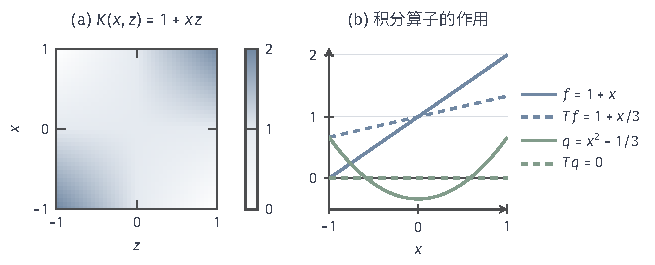
\includegraphics[width=110.9mm]{figures/02-abstract-mathematics/03-function-spaces/tikz/c3-kernel-action/figure.pdf}
  \caption{核$K(x,z)=1+xz$及其积分算子在$L^2([-1,1],dz/2)$上的作用。(a) 核的热图，颜色越深取值越大；沿对角方向$xz>0$时权重大于$1$。(b) $f=1+x$被映为$Tf=1+x/3$，常数方向保留、线性方向乘$1/3$；与$1,x$都正交的$q=x^2-1/3$被映为零。}
  \label{fig:ose-kernel-action}
\end{figure}

图~\ref{fig:ose-kernel-action}把核与作用放在一起。左图中的权重随$x,z$同号或异号而增减，正是这种结构使输出只记住输入的“平均”和“倾斜”；右图中，$q$虽然不是零函数，却与两个被记住的方向都正交，因而完全被消去。用第~\ref{sec:ose-spectral-theorem}小节的语言，$1$与$\sqrt3x$是特征值$1$与$1/3$的特征函数，$q$属于无限维的核空间。由于输出落在二维空间$\operatorname{span}\{1,x\}$中，$T$是秩为$2$的有限秩算子；一般地，$K(y,x)=\sum_{i=1}^r\varphi_i(y)\psi_i(x)$这类分离变量的有限和总给出秩不超过$r$的积分算子。

\paragraph{测度是算子的一部分}
保持核公式不变，把测度换成Lebesgue测度$dz$，两个矩都加倍，算子变成
\[
  (\tilde Tf)(x)=\int_{-1}^{1}(1+xz)f(z)\,dz=2\int f\,d\mu+2x\int zf\,d\mu ,
\]
于是$\tilde T(1+x)=2+2x/3$，特征值变为$2$与$2/3$，单位特征函数也随新内积重新归一化。同一个核在不同测度下给出不同的算子，谱也随之改变；讨论积分算子的谱时，必须同时报告核和测度。

\subsection{平方可积核与紧性}
\label{sec:ose-hilbert-schmidt}

现在给出一个容易检查的条件，使公式~\eqref{eq:ose-integral-operator}定义$L^2(\mu)$到$L^2(\nu)$的有界算子，并进一步是紧算子。下面用到的乘积测度与一般测度空间上的Tonelli、Fubini定理见本卷第~\ref{sec:integral-iterated}节（定理~\ref{thm:analysis-tonelli-fubini}与定理~\ref{thm:integral-fubini}）。

\paragraph{有界性}
逐点看，$(Tf)(y)$是截面$K(y,\cdot)$与$f$的内积，Cauchy–Schwarz不等式控制它的大小；再对$y$平方积分，截面范数的平方积分恰好是核的$L^2$范数平方。

\begin{theorem}[平方可积核的有界性]
\label{thm:ose-hs-bounded}
设$(X,\mu)$、$(Y,\nu)$为$\sigma$有限测度空间，$K\in L^2(\nu\otimes\mu)$。则对每个$f\in L^2(\mu)$，积分~\eqref{eq:ose-integral-operator}对$\nu$几乎每个$y$绝对收敛，$Tf\in L^2(\nu)$，且
\begin{equation}
  \|Tf\|_{L^2(\nu)}\leq\|K\|_{L^2(\nu\otimes\mu)}\|f\|_{L^2(\mu)},\qquad\text{从而}\quad\|T\|\leq\|K\|_{L^2(\nu\otimes\mu)} .
  \label{eq:ose-hs-bound}
\end{equation}
\end{theorem}

\begin{proof}
第一步，取得平方可积的截面。对非负函数$|K|^2$用Tonelli定理，
\[
  \int_Y\Bigl(\int_X|K(y,x)|^2\,d\mu(x)\Bigr)d\nu(y)=\|K\|_{L^2(\nu\otimes\mu)}^2<\infty ,
\]
所以内层积分对$\nu$几乎每个$y$有限，即截面$K(y,\cdot)\in L^2(\mu)$几乎处处成立。

第二步，逐点估计。对这样的$y$，由Cauchy–Schwarz不等式，
\[
  \int_X|K(y,x)f(x)|\,d\mu(x)\leq\|K(y,\cdot)\|_{L^2(\mu)}\|f\|_{L^2(\mu)}<\infty ,
\]
积分绝对收敛，且$|(Tf)(y)|\leq\|K(y,\cdot)\|_{L^2(\mu)}\|f\|_{L^2(\mu)}$。可测性也由Fubini定理得到：在任一有限测度的可测集$E\subseteq Y$上，对上式关于$y$积分并再用一次Cauchy–Schwarz不等式，
\[
  \int_E\int_X|K(y,x)f(x)|\,d\mu(x)\,d\nu(y)\leq\nu(E)^{1/2}\|K\|_{L^2(\nu\otimes\mu)}\|f\|_{L^2(\mu)}<\infty ,
\]
所以$(y,x)\mapsto K(y,x)f(x)$在$E\times X$上可积，内层积分$y\mapsto(Tf)(y)$在$E$上可测；$Y$是可数个这样的集合之并。

第三步，对$y$积分。把第二步的逐点界平方后积分，
\[
  \|Tf\|_{L^2(\nu)}^2\leq\int_Y\|K(y,\cdot)\|_{L^2(\mu)}^2\,d\nu(y)\,\|f\|_{L^2(\mu)}^2=\|K\|_{L^2(\nu\otimes\mu)}^2\|f\|_{L^2(\mu)}^2 .
\]
线性显然，于是$T$是有界线性算子，且式~\eqref{eq:ose-hs-bound}成立。
\end{proof}

平方可积核给出的积分算子称为\term{Hilbert--Schmidt积分算子}（Hilbert--Schmidt integral operator）。在贯穿例子中，
\[
  \|K\|_{L^2(\mu\otimes\mu)}^2=\iint(1+xz)^2\,d\mu(x)\,d\mu(z)=1+2\cdot0+\tfrac13\cdot\tfrac13=\tfrac{10}{9},
\]
而$\|T\|=1$（最大特征值），确实满足$\|T\|\leq\sqrt{10/9}$。注意$10/9=1^2+(1/3)^2$恰好是特征值的平方和；对例~\ref{ex:ose-volterra-svd}的积分算子$V$，$\|\mathbf 1_{\{t<x\}}\|_{L^2}^2=1/2$，而$\sum_k\sigma_k^2=\frac{4}{\pi^2}\sum_k\frac{1}{(2k-1)^2}=\frac{4}{\pi^2}\cdot\frac{\pi^2}{8}=\frac12$。可以证明，核的$L^2$范数平方总等于奇异值的平方和，这里只把它作为两个例子中的数值核对。

\paragraph{平方可积只是充分条件}
有界积分算子的核不必平方可积。取$X=Y=\mathbb N$，$\mu=\nu$为计数测度，此时$L^2$就是$\ell^2$，积分就是求和。核$K(m,n)=\mathbf 1_{\{m=n\}}$给出$(Tf)(m)=\sum_nK(m,n)f(n)=f(m)$，即单位算子，它有界而且范数为$1$；但$\|K\|_{L^2}^2=\sum_{m,n}K(m,n)^2$是无穷多个$1$之和，发散。由第~\ref{sec:ose-compact-def}小节，这个算子也不是紧算子。所以定理~\ref{thm:ose-hs-bounded}只说平方可积够用，不说有界算子都必须如此。

\paragraph{用矩形核逼近}
紧性的证明沿用第~\ref{sec:ose-finite-rank}小节的路线：把算子写成有限秩算子的算子范数极限。式~\eqref{eq:ose-hs-bound}说明核的$L^2$误差控制算子范数误差，所以只需用分离变量的有限和逼近核。最简单的分离变量核是矩形示性函数$\mathbf 1_{B\times A}(y,x)=\mathbf 1_B(y)\mathbf 1_A(x)$，下面的引理说明它们的线性组合足够用。

\begin{lemma}[矩形逼近]
\label{lem:ose-rectangle-approx}
设$(X,\mu)$、$(Y,\nu)$为有限测度空间，$E$属于乘积$\sigma$代数。则对每个$\varepsilon>0$，存在有限个两两不交的可测矩形$B_i\times A_i$，其并$R$满足$(\nu\otimes\mu)(E\,\triangle\,R)<\varepsilon$。
\end{lemma}

\begin{proof}[证明（补充阅读）]
记$m=\nu\otimes\mu$，令$\mathcal E$为具有引理性质的可测集全体。可测矩形显然在$\mathcal E$中。有限个矩形的不交并组成的族$\mathcal R$对有限交、补和有限并封闭：两个矩形之交仍是矩形，$(B\times A)^c=(B^c\times X)\cup(B\times A^c)$是两个不交矩形之并。

若$E\in\mathcal E$，取$R\in\mathcal R$逼近它，则$R^c\in\mathcal R$且$E^c\triangle R^c=E\triangle R$，所以$\mathcal E$对补封闭。若$E_1,E_2,\ldots\in\mathcal E$，令$E=\bigcup_kE_k$。总测度有限，故可取$N$使$m(E\setminus\bigcup_{k\leq N}E_k)<\varepsilon/2$；再对$k\leq N$取$R_k\in\mathcal R$使$m(E_k\triangle R_k)<\varepsilon/(2N)$。令$R=\bigcup_{k\leq N}R_k\in\mathcal R$，则
\[
  m(E\triangle R)\leq m\Bigl(E\setminus\bigcup_{k\leq N}E_k\Bigr)+\sum_{k\leq N}m(E_k\triangle R_k)<\varepsilon ,
\]
所以$\mathcal E$对可数并封闭。$\mathcal E$是包含全部可测矩形的$\sigma$代数，因而包含它们生成的乘积$\sigma$代数。
\end{proof}

\begin{theorem}[平方可积核给出紧算子]
\label{thm:ose-hs-compact}
在定理~\ref{thm:ose-hs-bounded}的条件下，$T:L^2(\mu)\to L^2(\nu)$是紧算子。
\end{theorem}

\begin{proof}
第一步，截断到有限测度区域。由$\sigma$有限性，取递增的可测集$X_k\uparrow X$、$Y_k\uparrow Y$，且$\mu(X_k),\nu(Y_k)<\infty$。令$K_k=K\mathbf 1_{Y_k\times X_k}$，则$|K-K_k|^2\leq|K|^2$且逐点趋于零，由控制收敛定理$\|K-K_k\|_{L^2}\to0$。

第二步，在有限测度区域内用简单函数逼近。由第~\ref{sec:fs-density-separability}节，简单函数在$L^2$中稠密，所以$K_k$可以被形如$\sum_ic_i\mathbf 1_{E_i}$的简单函数以任意精度逼近，其中$E_i\subseteq Y_k\times X_k$可测。由引理~\ref{lem:ose-rectangle-approx}，每个$\mathbf 1_{E_i}$又可以被有限个矩形示性函数之和逼近，且$\|\mathbf 1_{E_i}-\mathbf 1_{R_i}\|_{L^2}=m(E_i\triangle R_i)^{1/2}$。综合两步，对每个$\varepsilon>0$，存在形如
\[
  K_\varepsilon(y,x)=\sum_{i=1}^{r}c_i\mathbf 1_{B_i}(y)\mathbf 1_{A_i}(x)
\]
的核，使$\|K-K_\varepsilon\|_{L^2(\nu\otimes\mu)}<\varepsilon$。

第三步，回到算子。核$K_\varepsilon$对应的积分算子把$f$送到$\sum_ic_i\bigl(\int_{A_i}f\,d\mu\bigr)\mathbf 1_{B_i}$，像落在$\operatorname{span}\{\mathbf 1_{B_1},\ldots,\mathbf 1_{B_r}\}$中，是有限秩算子。对核差$K-K_\varepsilon$应用式~\eqref{eq:ose-hs-bound}，算子范数误差不超过$\varepsilon$。由定理~\ref{thm:ose-compact-limit}，$T$是紧算子。
\end{proof}

\begin{figure}[!htb]
  \centering
  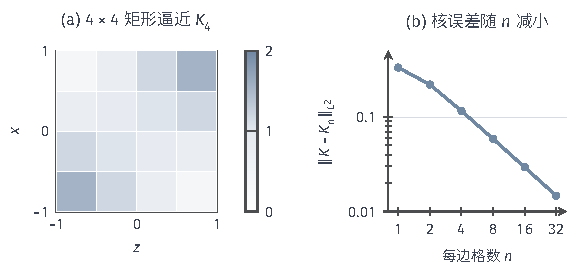
\includegraphics[width=97.4mm]{figures/02-abstract-mathematics/03-function-spaces/tikz/c3-rectangle-kernel/figure.pdf}
  \caption{用矩形示性函数的线性组合逼近核$K(x,z)=1+xz$（测度$dz/2$的乘积）。(a) $4\times4$均匀网格上取格内平均得到的分片常数核$K_4$，每格对应一个矩形$B_i\times A_j$。(b) $n\times n$网格平均的误差$\|K-K_n\|_{L^2}$，从$n=1$时的$1/3$降到$n=32$时约$0.015$，大致按$1/n$下降；它同时是相应有限秩算子的算子范数误差上界。}
  \label{fig:ose-rectangle-kernel}
\end{figure}

图~\ref{fig:ose-rectangle-kernel}在贯穿例子上演示第二步。用$n\times n$网格上的格内平均作分片常数核$K_n$，它是$n^2$个矩形示性函数的线性组合，对应的积分算子秩不超过$n$。格宽为$h=2/n$时，误差平方等于各格中$(xz-\bar x_i\bar z_j)^2$的平均，其中$\bar x_i,\bar z_j$为格中心；直接计算得$n=1,2,4,8$时误差约为$0.333$、$0.220$、$0.116$、$0.059$。对这个核，分片常数逼近远不是最经济的：$K$本身秩为$2$，截断奇异值分解两项就精确。矩形逼近的价值在于它对任意平方可积核都可行，从而在不知道奇异值的情况下证明了紧性。

\subsection{核的对称性与算子伴随}
\label{sec:ose-kernel-symmetry}

第~\ref{sec:ose-spectral-theorem}小节的谱分解要求算子自伴。本小节说明，对平方可积核，伴随算子仍是积分算子，其核由原核交换变量并取共轭得到；由此可以直接从核判断自伴性。

\paragraph{伴随核}
伴随由等式$\langle g,Tf\rangle=\langle T^*g,f\rangle$确定。左边是一个二重积分，只要能交换积分次序，就可以把对$y$的积分移到$g$一侧，读出$T^*g$的公式。

\begin{theorem}[伴随核]
\label{thm:ose-adjoint-kernel}
在定理~\ref{thm:ose-hs-bounded}的条件下，$T:L^2(\mu)\to L^2(\nu)$的伴随$T^*:L^2(\nu)\to L^2(\mu)$是以
\[
  K^*(x,y)=\overline{K(y,x)}
\]
为核的积分算子，即$(T^*g)(x)=\int_Y\overline{K(y,x)}g(y)\,d\nu(y)$。
\end{theorem}

\begin{proof}
任取$f\in L^2(\mu)$、$g\in L^2(\nu)$。函数$(y,x)\mapsto|g(y)||K(y,x)||f(x)|$在乘积空间上可积：由乘积空间中的Cauchy–Schwarz不等式，它的积分不超过$\|K\|_{L^2}$乘以$(y,x)\mapsto|g(y)f(x)|$的$L^2$范数，后者由Tonelli定理等于$\|g\|\|f\|$。于是可以用Fubini定理交换积分次序：
\[
  \begin{aligned}
  \langle g,Tf\rangle&=\int_Y\overline{g(y)}\int_XK(y,x)f(x)\,d\mu(x)\,d\nu(y)\\
  &=\int_X\overline{\Bigl(\int_Y\overline{K(y,x)}g(y)\,d\nu(y)\Bigr)}f(x)\,d\mu(x).
  \end{aligned}
\]
括号中的函数正是以$K^*$为核的积分算子作用于$g$，且$K^*\in L^2(\mu\otimes\nu)$，由定理~\ref{thm:ose-hs-bounded}它属于$L^2(\mu)$。上式说明它满足伴随的定义式$\langle g,Tf\rangle=\langle T^*g,f\rangle$；由伴随的唯一性，它就是$T^*g$。
\end{proof}

伴随核把原核的输入、输出两个变量互换，在实值情形下就是关于对角线作镜像。图~\ref{fig:ose-kernel-adjoint}以例~\ref{ex:ose-volterra-svd}中的积分算子为例：$K(x,t)=\mathbf 1_{\{t<x\}}$在对角线上方取一，表示$(Vf)(x)$累积$x$左边的输入；伴随核在对角线下方取一，表示$(V^*g)(t)=\int_t^1g$累积$t$右边的输入。这正是例中通过交换积分次序得到的公式。

\begin{figure}[!htb]
  \centering
  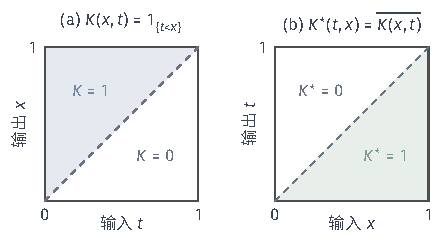
\includegraphics[width=75.2mm]{figures/02-abstract-mathematics/03-function-spaces/tikz/c3-kernel-adjoint/figure.pdf}
  \caption{积分核与伴随核关于对角线互为镜像。(a) $(Vf)(x)=\int_0^xf$的核$K(x,t)=\mathbf 1_{\{t<x\}}$，纵轴为输出变量，阴影处取值$1$。(b) 伴随核$K^*(t,x)=\overline{K(x,t)}=\mathbf 1_{\{x>t\}}$，给出$(V^*g)(t)=\int_t^1g$。两核不相等，所以$V$不自伴。}
  \label{fig:ose-kernel-adjoint}
\end{figure}

\paragraph{对称核与自伴}
当$X=Y$且$\mu=\nu$时，若$K(x,z)=\overline{K(z,x)}$对$\mu\otimes\mu$几乎处处的$(x,z)$成立，则$K^*=K$几乎处处，由定理~\ref{thm:ose-adjoint-kernel}得$T^*=T$，$T$是紧自伴算子。这时定理~\ref{thm:ose-compact-selfadjoint}的谱分解可以直接使用。实值核的这一条件就是对称性$K(x,z)=K(z,x)$。贯穿例子的$1+xz$是实对称核，所以它的特征函数$1$与$\sqrt3x$正交、特征值是实数，与第~\ref{sec:ose-spectral-theorem}小节的计算一致；积分算子$V$的核不对称，它的左右奇异函数是两组不同的三角函数。

\paragraph{对称不等于正}
自伴只说明二次型$\langle f,Tf\rangle$是实数，并不保证它非负。核$1-6xz$实对称，但取$f=x$得$Tf=-2x$，
\[
  \langle f,Tf\rangle=\int x\cdot(-2x)\,d\mu=-\tfrac23<0 .
\]
相比之下，$1+xz$给出$\langle f,Tf\rangle=|\int f\,d\mu|^2+|\int xf\,d\mu|^2\geq0$，是正算子。正性要单独检查，不能从核对称推出。

\paragraph{等价类与点值}
平方可积核本身只是$\nu\otimes\mu$几乎处处的等价类。在零测集上改动核不改变积分算子，却可能完全改变它在个别点上的取值。例如在$[-1,1]^2$上令$K'(x,z)=1+xz-10\cdot\mathbf 1_{\{x=z\}}$，对角线在乘积测度下为零测集，所以$K'$与$K$给出同一个正算子；但$K'(x,x)=x^2-9<0$，单点$\{x\}$上的$1\times1$“Gram矩阵”为负。因此，从本节的$L^2$结论出发，不能谈论“所有有限点集上的Gram矩阵是否半正定”，也不能谈论核在指定点上的再生关系。这些问题需要核取连续代表、并对所有有限点集半正定，属于第~\ref{sec:rkhs-point-evaluation}节及第~\ref{sec:rkhs-mercer}节的内容。
